\documentclass[11pt]{article}

\usepackage{caption}
\usepackage{graphicx}
\usepackage{booktabs}
\usepackage[margin=0.88in]{geometry}
\usepackage{amsmath}
\usepackage{titlesec}
\usepackage{enumerate}
\usepackage{bm}
\usepackage{subfig}

\setlength{\parindent}{0pt}

\begin{document}
	\begin{titlepage}
	\begin{flushleft}
	Imperial College London \\
	Department of Aeronautics \\
	Third Year HPC Coursework Report 2020 \\
	\end{flushleft}
	\vspace*{\fill}	
	\begin{center}
		\textsc{\Huge High Performance Computing Coursework} \\
		\vspace{11pt}
		\textit{\small Done by:} \\
		\textsc{\Large Chai Jun, Sean} \\
		\textsc{CID: 01327446} \\ 
		\vspace*{\fill}
	\end{center}
		
	\end{titlepage}
	
	\tableofcontents
	\newpage
	
	\section{Result of running Lid Driven Cavity Solver}
	\subsection{Velocity Plots}
	\begin{figure}[htp]
            \centering
            \subfloat[Horizontal velocity $u$ against $x$ along $y=0.5$]{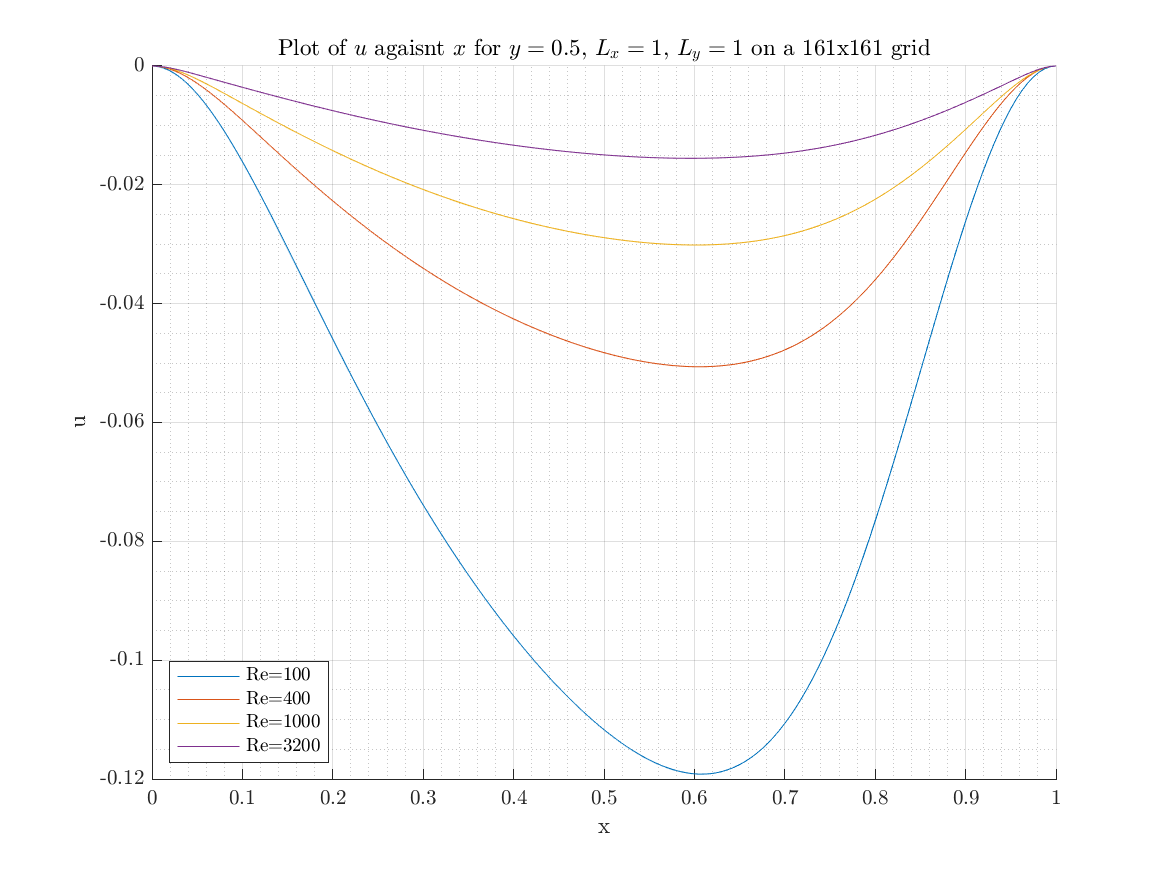
\includegraphics[width=0.48\textwidth]{../Images/u_vs_x.png}}
            \hfill
            \subfloat[Vertical velocity $v$ against $y$ along $x=0.5$]{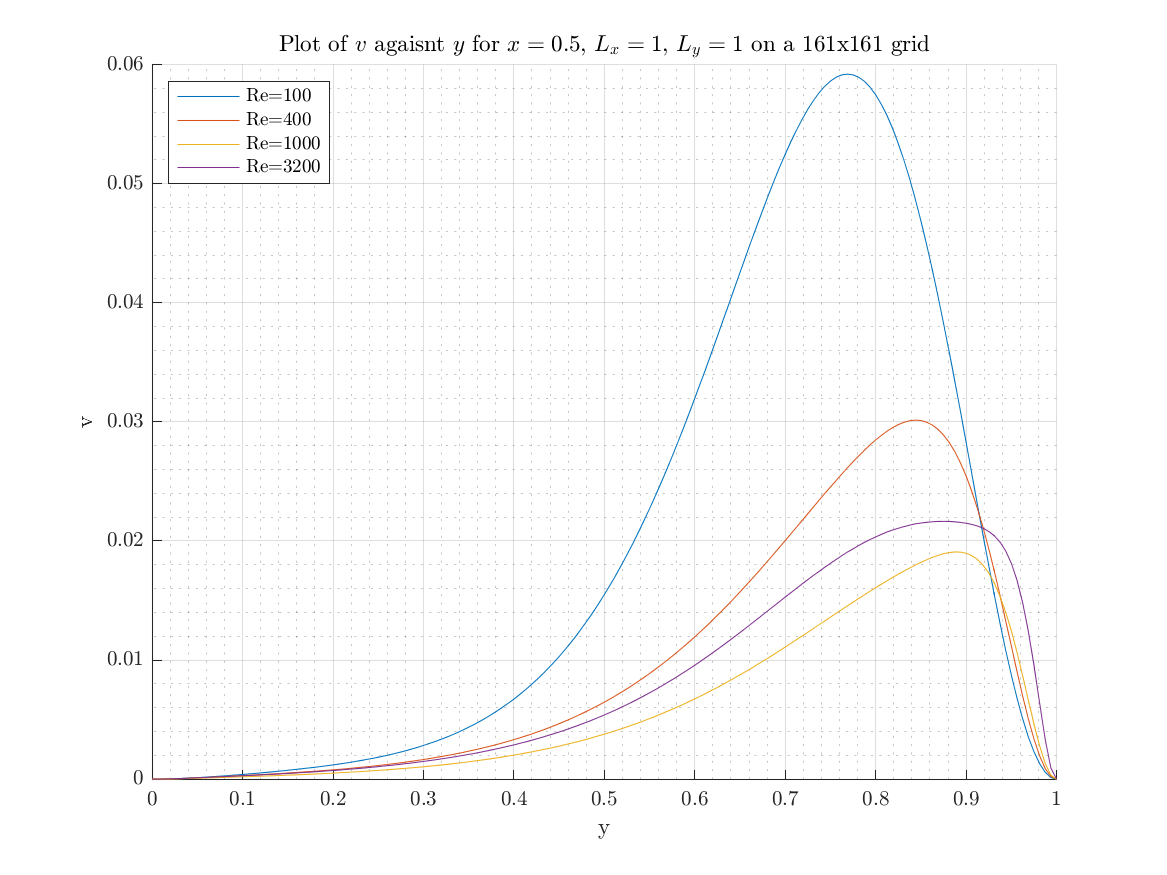
\includegraphics[width=0.48\textwidth]{../Images/v_vs_y.png}}
            \caption{Plot of velocities of the steady state solution for Reynolds numbers of 100, 400, 1000 and 3200 using a $161 \times 161$ grid and $L_x = L_y = 1$.}
            \label{fig:velocities}
        \end{figure}
	
	\subsection{Vorticity and Streamfunction}
	\begin{figure}[htp]
            \centering
            \subfloat[Vorticity contour plot]{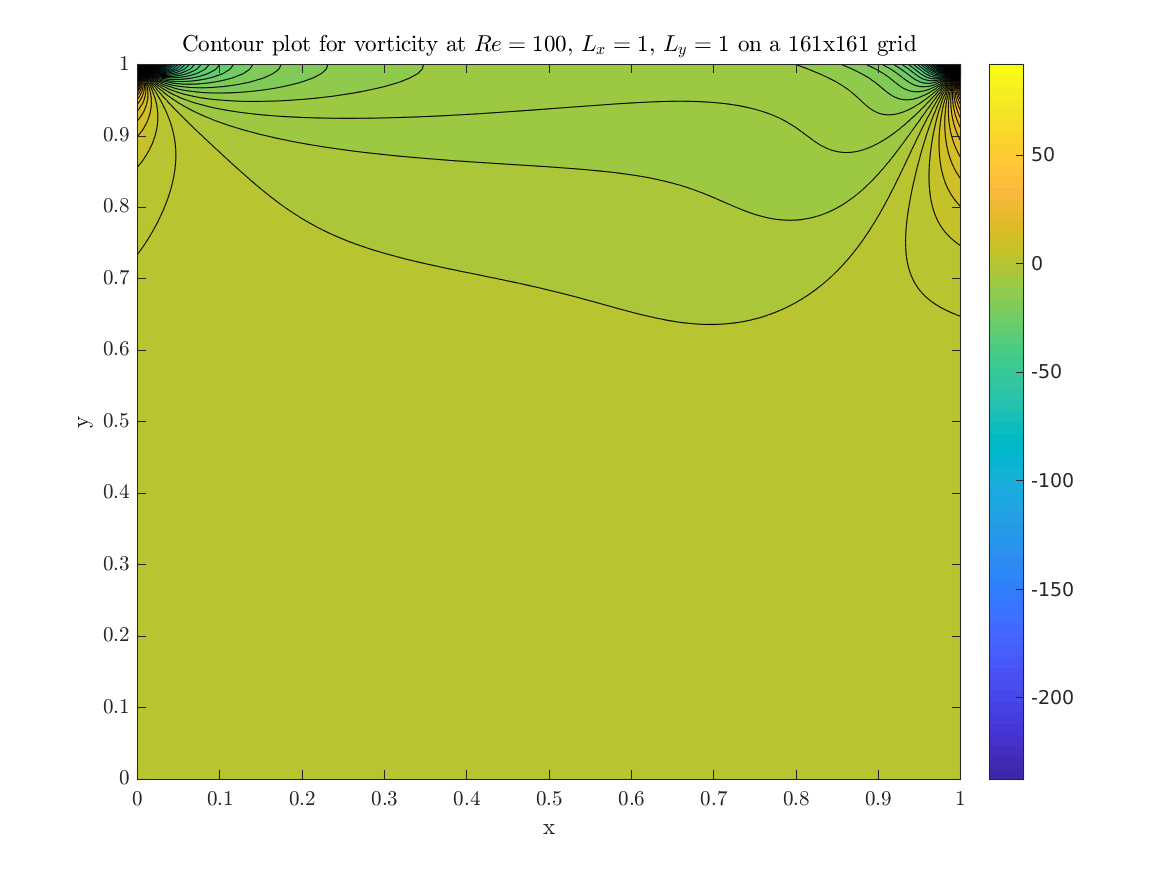
\includegraphics[width=0.48\textwidth]{../Images/w_100.png}}
            \hfill
            \subfloat[Streamfunction contour plot]{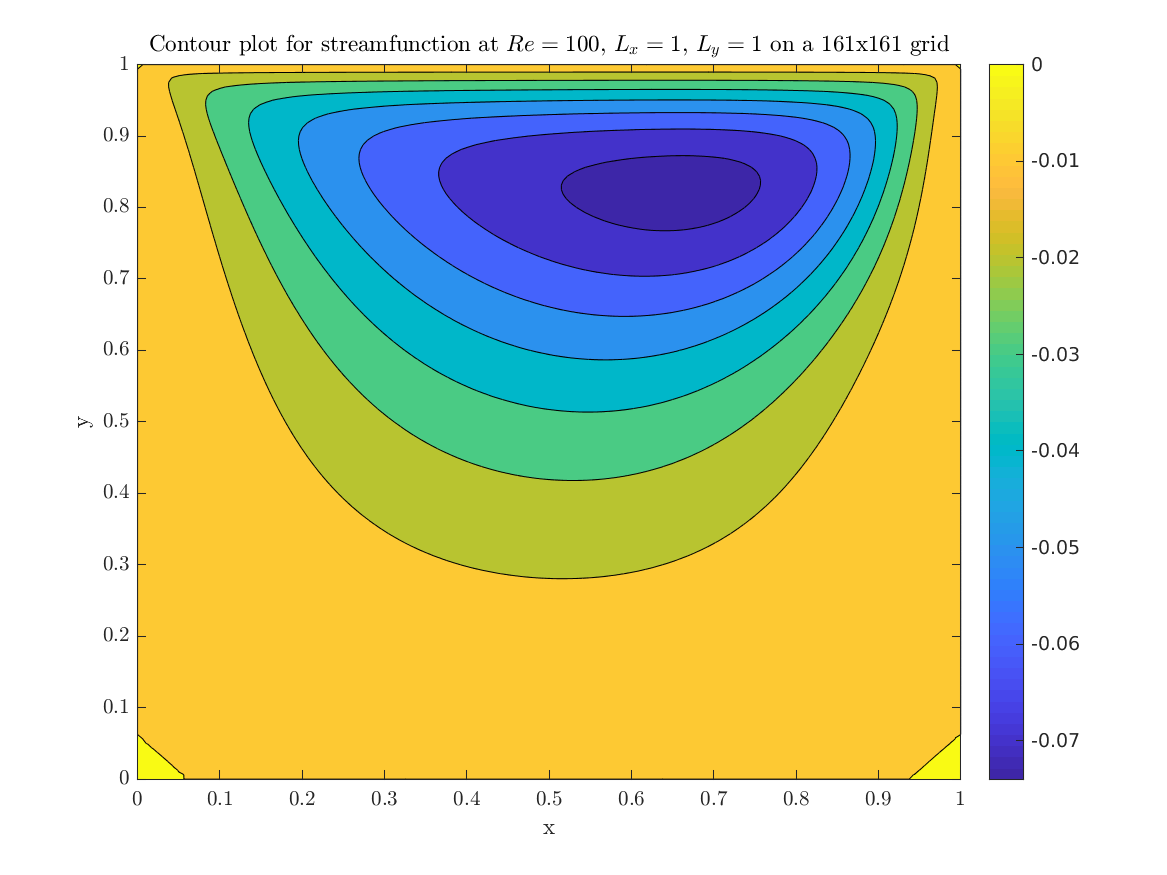
\includegraphics[width=0.48\textwidth]{../Images/s_100.png}}
            \caption{Contour plots of vorticity and streamfunction at $Re=100$ on a $161 \times 161$ grid and $L_x = L_y = 1$.}
            \label{fig:contours}
        \end{figure}			
	
	\newpage
	\subsection{Minimum Streamfunction}
	\begin{table}[htb]
    	\centering
    	\begin{tabular}{ c | c c c c }
    	\toprule
    	Reynolds Number & 100 & 400 & 1000 & 3200 \\
    	\midrule
		x-coordinate &  &  &  &  \\
		y-coordinate &  &  &  &  \\
        \bottomrule
        \end{tabular}
        \vspace{0.5em}
        \label{tab:stress}
    	\caption{Table of x-y coordinates of the streamfunction minimum at the different Reynolds numbers for a $161 \times 161$ grid and $L_x = L_y = 1$.}	
	\end{table}
	
	\subsection{Streamfunction Plots for Varying $L_x$ and $L_y$}
	\begin{figure}[htb]
		\centering
		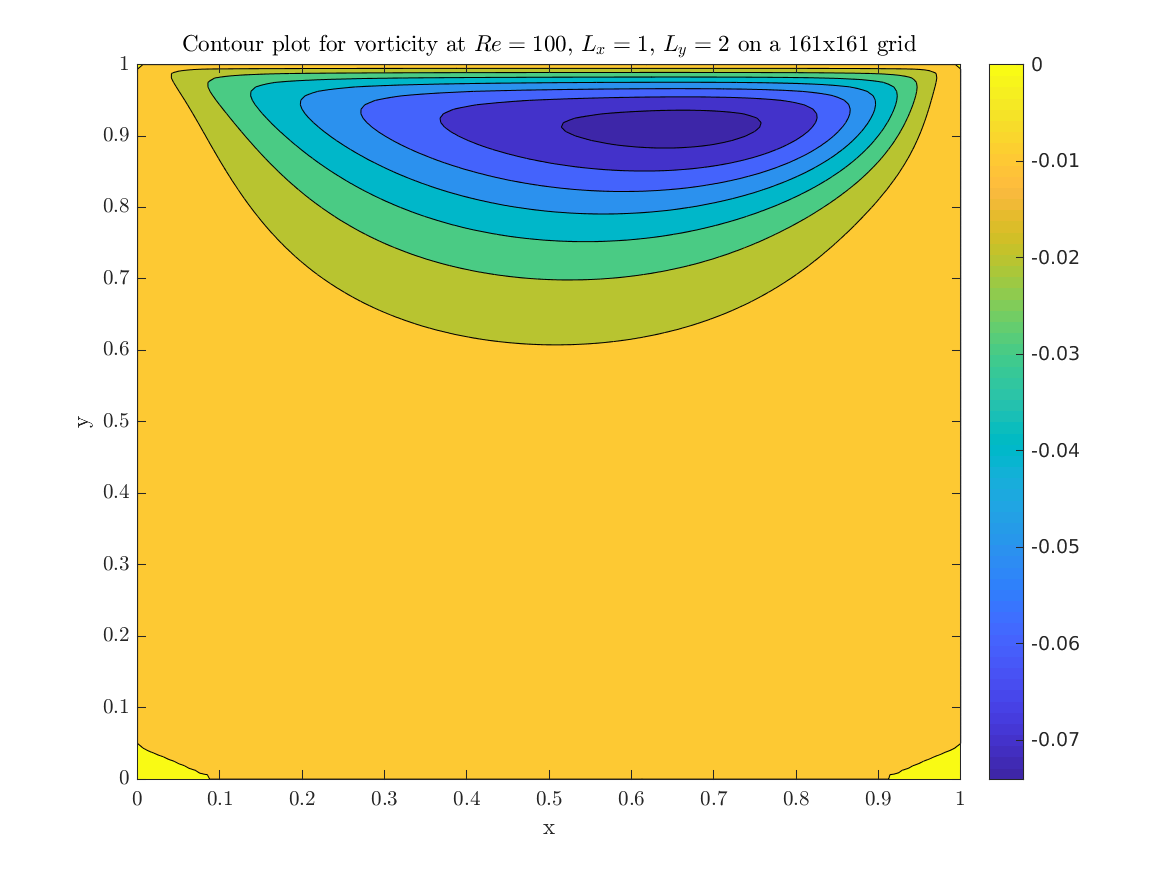
\includegraphics[width=\linewidth]{../Images/lx1ly2.png}
		\captionof{figure}{Contour plot of streamfunction at $Re=100$ on a $161 \times 161$ grid and $L_x = 1, \, L_y = 2$.}
  		\label{fig:s_100}
	\end{figure}
	
	\begin{figure}[htb]
		\centering
		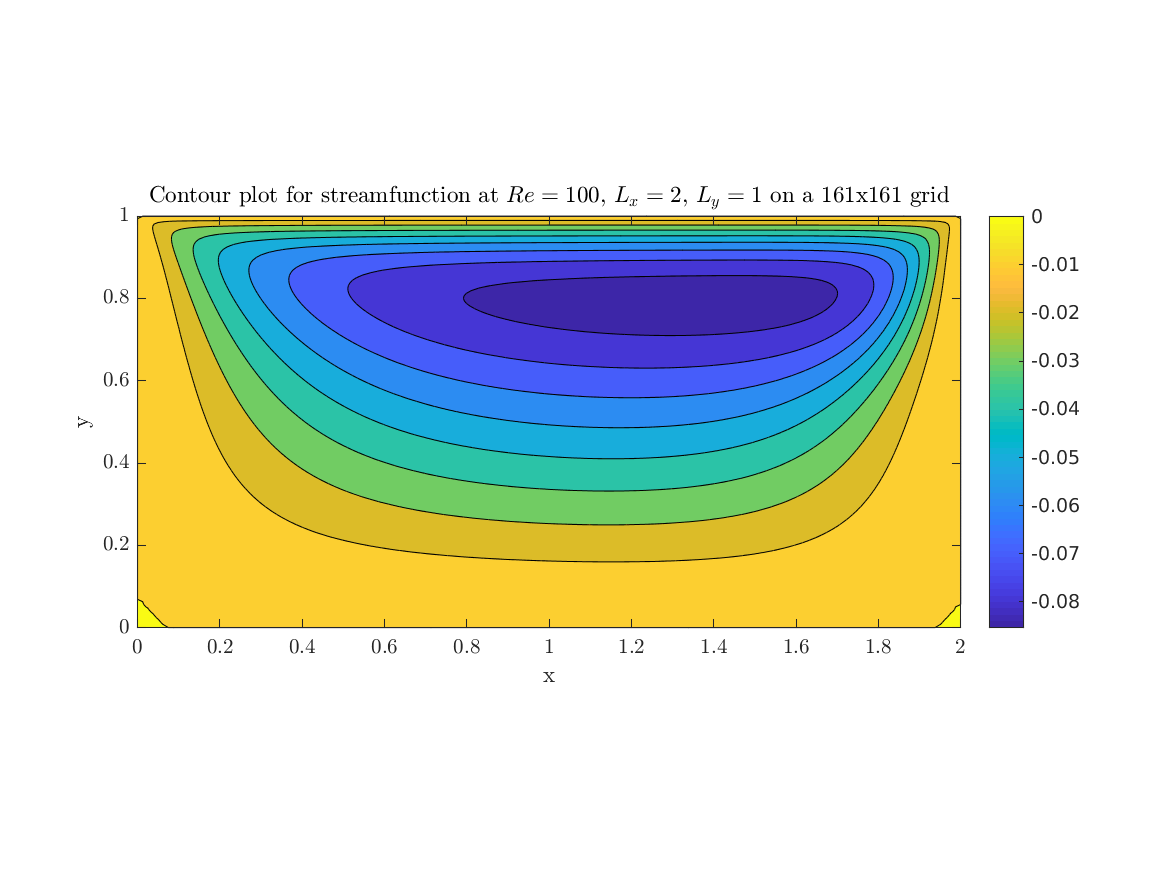
\includegraphics[width=\linewidth]{../Images/lx2ly1.png}
		\captionof{figure}{Contour plot of streamfunction at $Re=100$ on a $161 \times 161$ grid and $L_x = 2, \, L_y = 1$.}
  		\label{fig:lx2ly1}
	\end{figure}
	
	\section{Discussion of Parallel Code}
	One key decision in implementing the code was to swap around the steps of the algorithm. Since the calculation of the inner vorticity and the boundary vorticity are independent of one another, we can swap the steps around. By calculating the interior vorticity before the boundary, it allowed for easier parallelising of code as the coded needed to be less careful in
	
	The updating of the boundary conditions was not parallelised as the time taken to send and receive the data take around the same time compared to just a simple ``for" loop. As such, the decision was made to not parallelise that portion of the code.
	
	One method of optimising the code was to do the update of vorticity at time $t$ and $t+dt$ in a manner that is consistent with the storage of the data. In our case, that meant updating the values in a column-major format as the matrices were stored as such. This allowed for faster memory access due to the reduced need of traversing through the array to reach the memory address. Additionally, I allocated the same chunk of the array to the same processes for the parallel portion of the code. This allowed each processor to access the same part of the array each time, thereby utilising memory caching which allowed for faster memory access.
	
	Another method of optimising the serial code was to separate it from the parallel one. This reduced the need to
\end{document}